%!TEX root = ../zeeman.tex

Некоторые закономерности эффекта Зеемана могут быть проиллюстрированы на классической модели, которая основывается на том, что движущийся вокруг ядра атома электрон обладает механическим и магнитным моментам связанными соотношением $\vec{\mu}_{l_i}=-\gamma \vec{P}_{l_i}$. Таким образом, классическая модель, в отличие от квантовой, не учитывает собственный механический момент (спин) и магнитный момент электрона и, следовательно, может дать верные результаты лишь в частном случае, когда спины электронов в атоме скомпенсированы ($s=0$). По чисто историческим причинам этот случай получил название \textbf{нормального} (или \textbf{простого}) \textbf{эффекта Зеемана}, тогда как при \textbf{$s\ne0$} эффект Зеемана называют \textbf{аномальным} (или \textbf{сложным}). 

\begin{wrapfigure}{h}{0.4\textwidth}
\begin{center}
\vspace{-50pt}
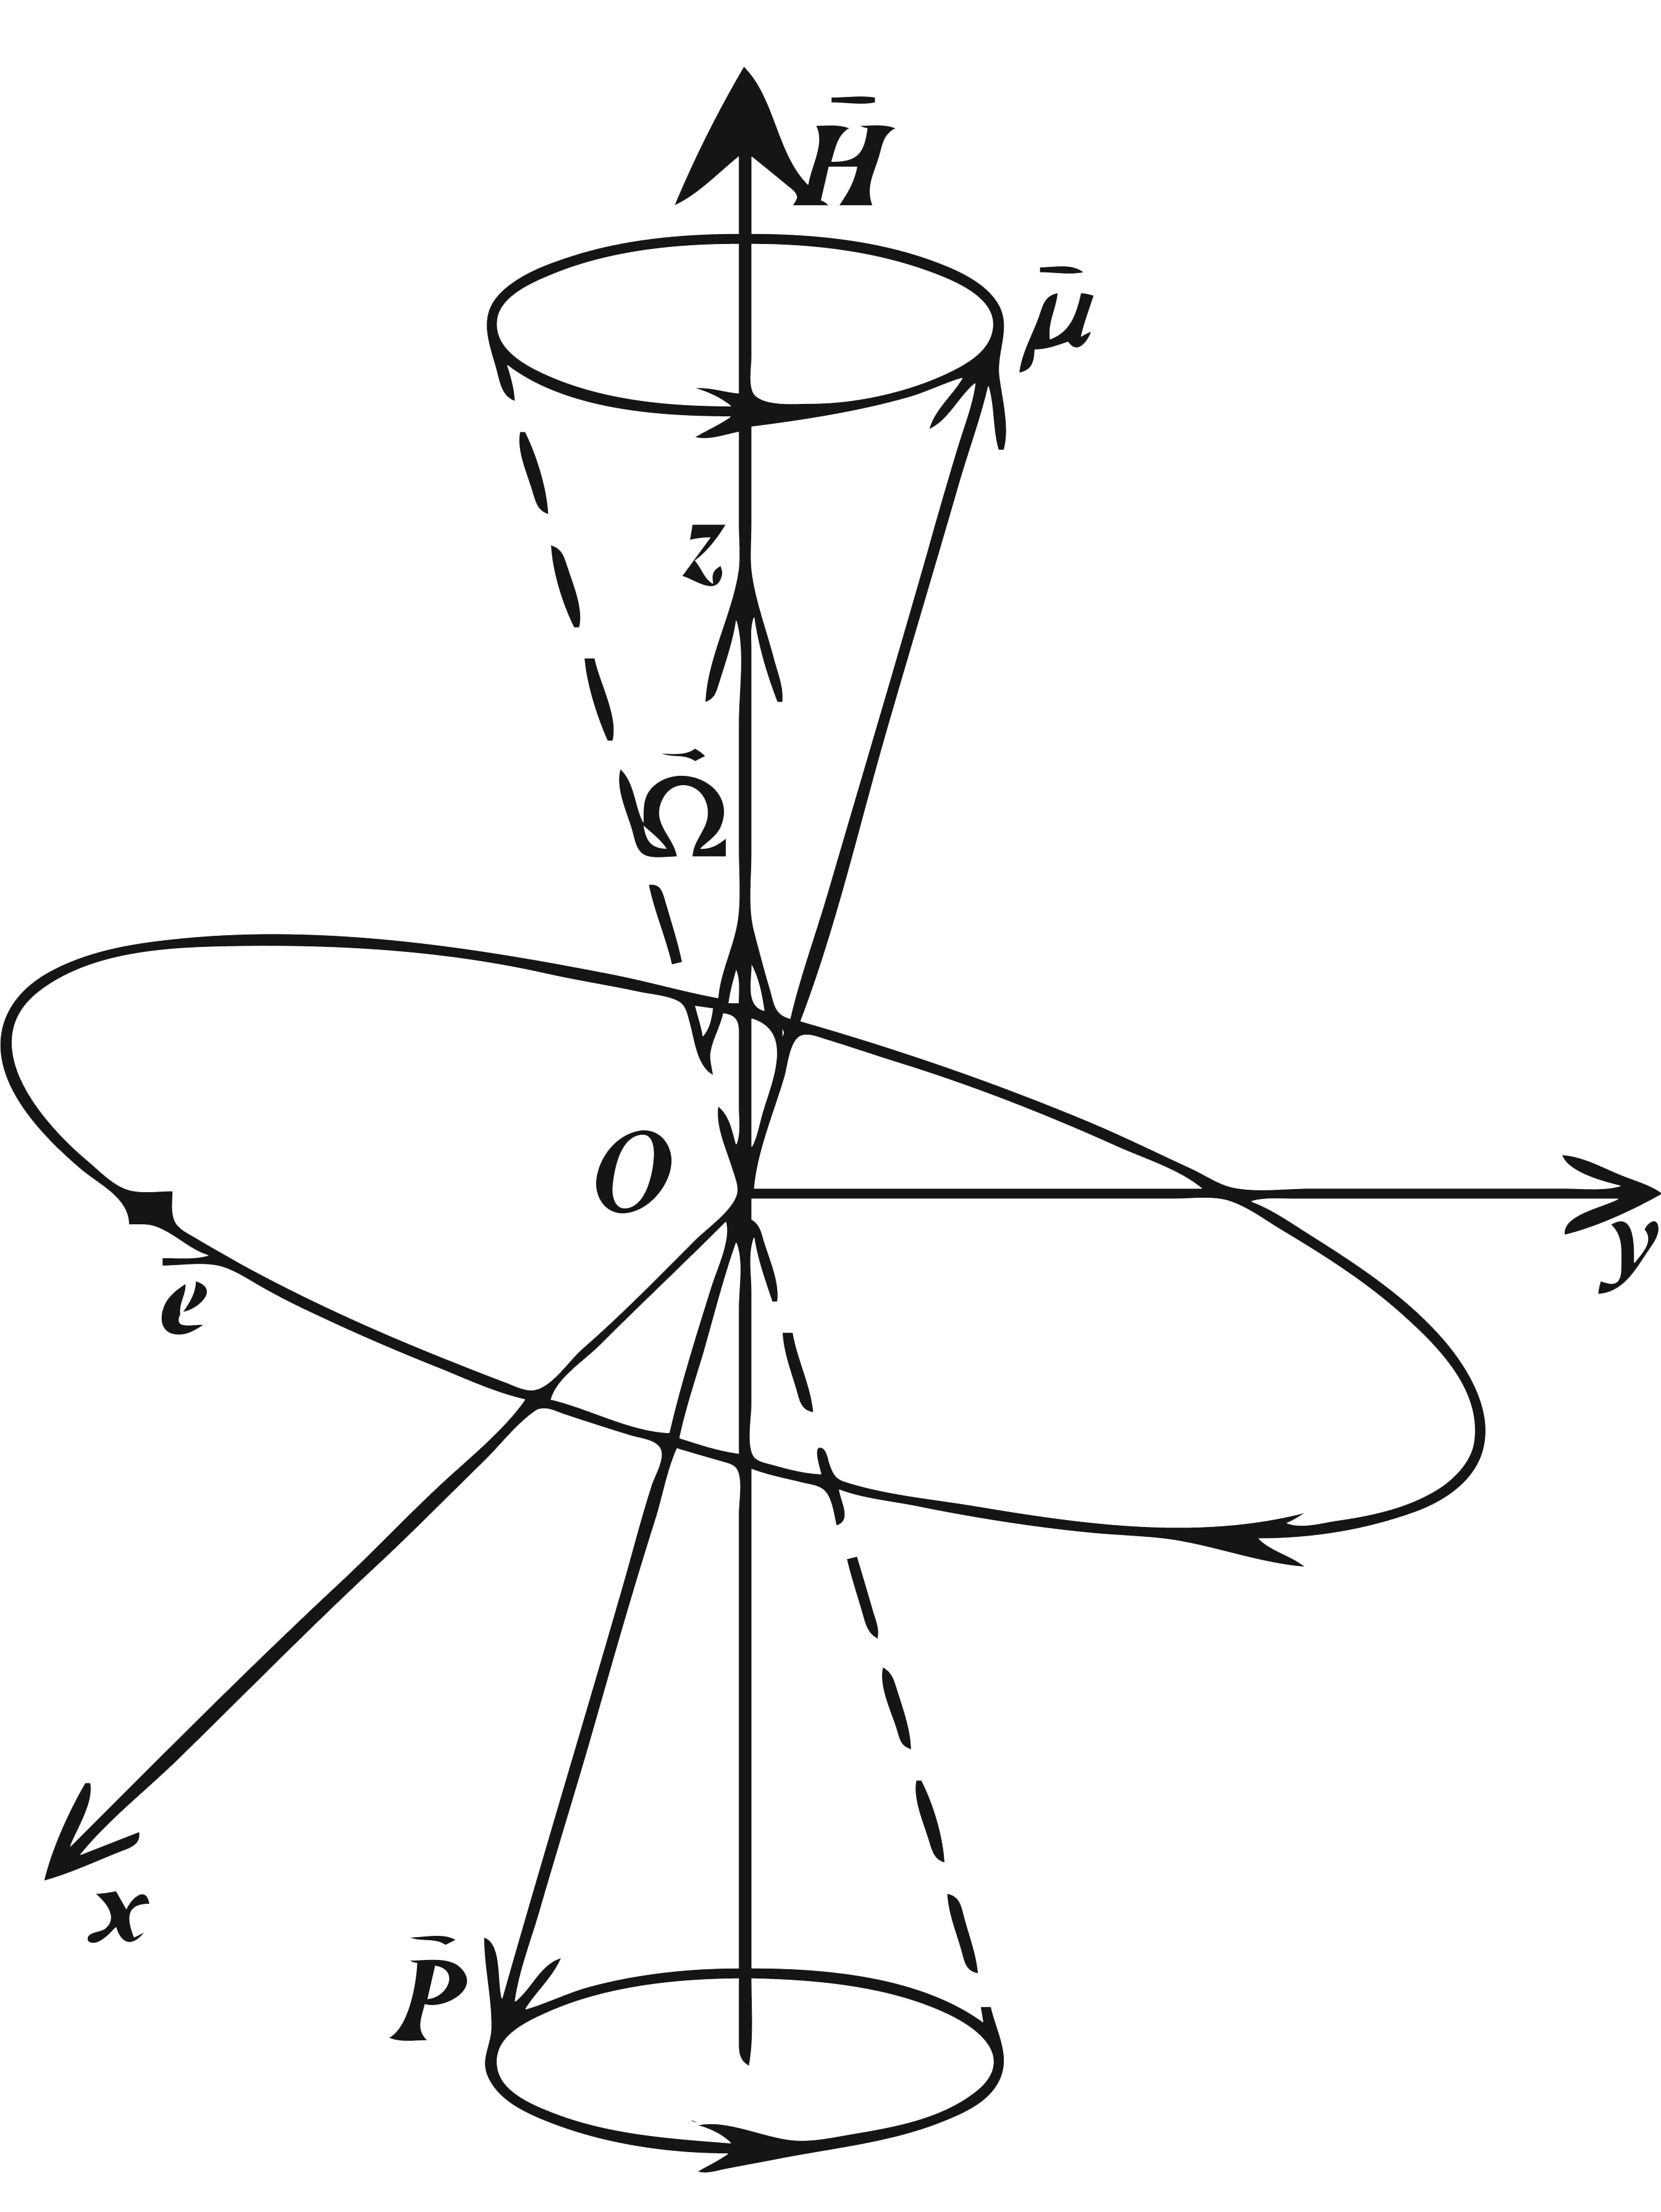
\includegraphics[width=0.4\textwidth]{fig/fig4.jpg}
\vspace{-45pt}
\end{center}
\caption{Прецессия электрона в магнитном поле классической модели атома}
\label{fig:4}
\end{wrapfigure}

Как легко показать из законов классической физики, орбитальный электронный ток (т.е. магнитный волчок) во внешнем магнитном поле прецессирует вокруг направления $\vec{H}$ с ларморовской частотой: 
\begin{equation}
	\label{eq:22}
	\Omega=\gamma H=\frac{eH}{2mc}.
\end{equation} 
Чтобы объяснить спектральный состав, а также поляризацию нормальных зeемановских компонент, надо разложить сложное движение электрона на более простые составляющие.

Введем лабораторную систему отсчета ($x, y, z$) как показано на \ref{fig:4}магнитное поле $\vec{H}$ направлено по оси $z$, а плоскость ($x, y$)- перпендикулярна ему. 

Пусть сначала магнитное поле отсутствует, то есть $\Omega = 0$ - прецессионного движения нет. Орбитальное движение разложим на движение в плоскости ($x, y$) и вдоль оси $z$. Проекция кругового орбитального движения на плоскость ($x, y$) является движением по эллипсу, которое, в свою очередь, можно представить в виде суммы двух круговых вращений, как это показано на \ref{fig:5}. 

% \begin{wrapfigure}{h}{0.6\textwidth}
% \begin{center}
% \vspace{-10pt}
% 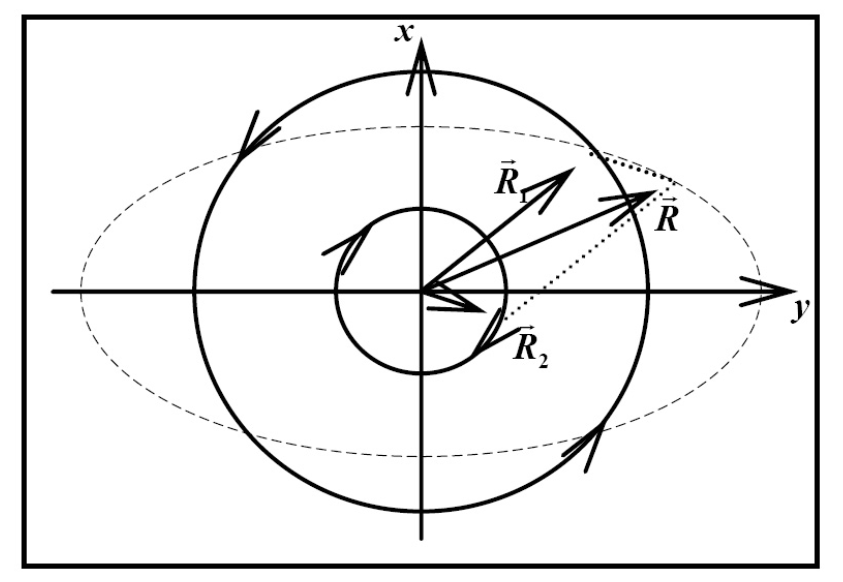
\includegraphics[width=0.6\textwidth]{fig/fig5.jpg}
% \vspace{-35pt}
% \end{center}
% \caption{Диаграмма, иллюстрирующая представление движения по эллипсу в виде суммы двух круговых}
% \label{fig:5}
% \end{wrapfigure}

\begin{figure}[tb]
	\centering
	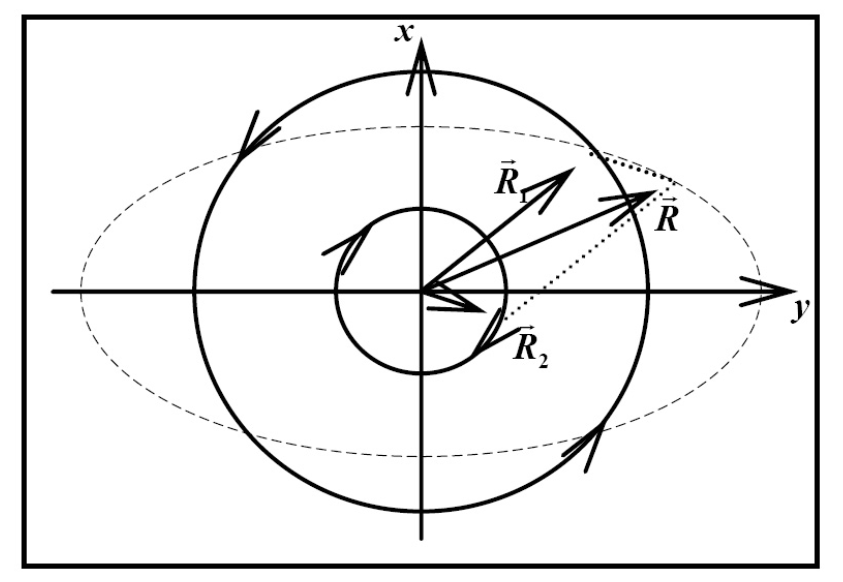
\includegraphics[width=0.6\textwidth]{fig/fig5.jpg}
	\caption{Диаграмма, иллюстрирующая представление движения по эллипсу в виде суммы двух круговых}
	\label{fig:5}
\end{figure}

Здесь вектора $\vec{R}_1$ и $\vec{R}_2$ вращаются в противоположных направлениях с угловой скоростью орбитального движения $\omega_0$ симметрично относительно большой оси эллипса, при этом конец вектора $\vec{R}$ двигается по эллипсу, большая полуось которого равна $|\vec{R}_1 + \vec{R}_2|$, а малая $|\vec{R}_1 - \vec{R}_2|$.

В свою очередь, разложив круговое орбитальное движение электрона на сумму двух линейных ортогональных гармонических колебаний, легко увидеть, что проекция этого движения на ось $z$ есть гармоническое колебание c частотой $\omega_0$.

При включении магнитного поля, как уже отмечалось выше, результирующее движение электрона будет суммой быстрого орбитального вращения и прецессии орбиты, то есть на орбитальное движение наложится вращение с угловой скоростью $\Omega$ вокруг оси $z$. Колебания вдоль оси $z$ при этом не изменятся, скорость вращения вектора $\vec{R}_1$ уменьшится, а вектора $\vec{R}_2$ увеличится на величину $\Omega$. 

Используя элементарную дипольную модель излучающего атома, легко увидеть что в спектре излучения вдоль направления внешнего магнитного поля будут присутствовать лишь две циркулярно поляризованные волны с частотами $\omega_{1,2}=\omega \pm \Omega$ (\textbf{нормальный зеeмановский дублет}), тогда как в перпендикулярном направлении будут наблюдаться три линейно поляризованные компоненты на частотах $\omega_1, \omega_0, \omega_2$ (\textbf{нормальный зеeмановский триплет}).

Поскольку расщепление линии обычно весьма мало, т.е. $|\omega_1 - \omega_2|\ll \omega_0$, из статистических соображений следует, что средняя кинетическая энергия каждой из трех составляющих движения (степеней свободы) электрона примерно одинакова. Это означает, что, если в отсутствие магнитного поля интенсивность линии излучения обозначить $I_0$, то интенсивности зеeмановских компонент составят $I_0/2$ и $I_0/2$ в дублете и $I_0/4, I_0/2, I_0/4$ в триплете. 

Таким образом, классическая теория предсказывает сам факт расщепления спектральных линий в магнитном поле, хорошо объясняет поляризацию излучения и качественно указывает на различную относительную интенсивность зеемановских компонент.
Число наблюдаемых зеемановских линий, их частоты и относительные интенсивности должны рассчитываться по приведенным выше квантомеханическим формулам.

